\documentclass[11pt]{article}

\usepackage[a4paper,margin=1in]{geometry}
\usepackage[T1]{fontenc}
\usepackage[utf8]{inputenc}
\usepackage{lmodern}
\usepackage{graphicx}
\usepackage{subcaption}
\usepackage{booktabs}
\usepackage{hyperref}
\usepackage{float}
\usepackage{longtable}
\usepackage{array}

\newcolumntype{L}[1]{>{\raggedright\arraybackslash}p{#1}}
\setcounter{table}{0}
\renewcommand{\thetable}{S\arabic{table}}
\setcounter{figure}{0}
\renewcommand{\thefigure}{S\arabic{figure}}

\title{Supplementary Material: City1 v2}
\author{}
\date{}

\begin{document}

\maketitle

\section*{Supplement overview}

This supplement contains the validation-evidence synthesis table, frozen technical appendices, detailed qualitative case panels, additional example surface maps, and expanded supporting tables referenced by the frozen City1 v2 manuscript package.

\section{S1. Validation-Evidence Matrix}

Supplementary Table~S1 summarizes the logic of the frozen validation stack. Its purpose is to make explicit what each layer supports, and just as importantly, what it does not support.

\begingroup
\small
\setlength{\LTleft}{0pt}
\setlength{\LTright}{0pt}
\begin{longtable}{L{0.14\textwidth} L{0.18\textwidth} L{0.16\textwidth} L{0.20\textwidth} L{0.22\textwidth}}
\caption{Validation-evidence matrix for the frozen City1 v2 manuscript. The table makes explicit what each layer contributes to credibility and what it does not establish.}\label{tab:s1_validation_matrix}\\
\toprule
Validation layer & Question answered & Metric / artifact used & What it supports & What it does not support \\
\midrule
\endfirsthead
\toprule
Validation layer & Question answered & Metric / artifact used & What it supports & What it does not support \\
\midrule
\endhead
\bottomrule
\endfoot
LOCO & Does the baseline transfer to unseen cities? & Calibrated RMSE and calibrated $R^2$ across hold-out cities & Cross-city transferability under data scarcity & Within-city local correctness or cell-level truth \\
Spatial block CV & Does performance remain stable when local leakage is restricted? & Blocked within-city cross-validation metrics & Within-city robustness under stricter spatial separation & Transfer to unseen cities or truth validation \\
Grid benchmark & Which operating resolution best balances detail and stability? & Benchmark score across 250 m, 500 m, and 1000 m grids & Frozen production choice for the main operating grid & A universal claim that one grid size is optimal in every setting \\
OSM completeness & How much open-data support is available by city? & Completeness score, label, and layer zero-share diagnostics & Interpretation confidence and caution context & Predictive accuracy or validation against population truth \\
District benchmark & Does the surface remain coherent after aggregation to available districts? & District-level Pearson and Spearman correlations & Partial internal administrative coherence where references exist & Cell-level truth validation or uniform reliability across cities \\
External benchmark & Do independent products agree with broad structure or hotspots? & Pearson, Spearman, top-decile overlap, hotspot IoU & External structural plausibility from independent gridded products & Ground-truth validation or proof that an external product is correct \\
Ablation & Which feature families carry the dominant share of predictive structure? & LOCO RMSE and $R^2$ by ablation family & Dependence on built form, marginal value of broader features, and role of calibration & Feature-level causality or a full explainability layer \\
Qualitative plausibility & Do curated hotspot and coldspot cases look urban-structurally plausible? & Overview maps and detailed curated case panels & Map interpretability and urban-structural plausibility & Quantitative validation or census-equivalent truth claims \\
\end{longtable}
\endgroup


\section{S2. City Registry and Coverage}

Supplementary Table~S2 gives the full frozen registry, distinguishes validated baseline cities from smoke-passed or runtime-only examples, and records the provenance route used for official totals.

\begingroup
\small
\setlength{\LTleft}{0pt}
\setlength{\LTright}{0pt}
\begin{longtable}{L{0.14\textwidth} L{0.20\textwidth} L{0.20\textwidth} L{0.12\textwidth} L{0.12\textwidth} L{0.12\textwidth}}
\caption{Frozen city registry and coverage in City1 v2. Completeness context is shown only where feature generation was available in the frozen package.}\label{tab:s2_registry}\\
\toprule
City & Frozen role & Official totals provenance & District benchmark & Qualitative anchor & Completeness context \\
\midrule
\endfirsthead
\toprule
City & Frozen role & Official totals provenance & District benchmark & Qualitative anchor & Completeness context \\
\midrule
\endhead
\bottomrule
\endfoot
Almaty & validated baseline city & manual verified BNS record & yes & yes & good \\
Astana & validated baseline city & manual verified BNS record & yes & yes & moderate \\
Shymkent & validated baseline city & manual verified BNS record & yes & no & moderate \\
Semey & validated baseline city; smoke-passed example & workbook-derived BNS record & no & no & good \\
Taraz & validated baseline city & workbook-derived BNS record & no & no & good \\
Uralsk & validated baseline city & workbook-derived BNS record & no & no & good \\
Petropavlovsk & validated baseline city & workbook-derived BNS record & no & no & good \\
Ust Kamenogorsk & validated baseline city & workbook-derived BNS record & no & no & good \\
Kurchatov & runtime-only calibrated example & workbook-derived BNS record & no & no & n/a \\
Ridder & official-total registry only & workbook-derived BNS record & no & no & n/a \\
\end{longtable}
\endgroup


\section{S3. Frozen Feature Inventory and Weak-Target Construction}

Supplementary Table~S3 lists the exact frozen model features by family and indicates whether each feature participates directly in the default weak-label construction.

\input{tables_tex/table_s3_feature_inventory.tex}

Let $x_{ik}$ denote feature $k$ for cell $i$, and let $K$ denote the weak-label feature subset available in city $c$. In the frozen workflow, negative values are clipped before transformation, the remaining values are log-transformed with $\log(1+x)$, and each feature is min-max normalized before fixed weights are applied:
\[
s_i = \sum_{k \in K} w_k \cdot \mathrm{MinMax}\!\left(\log\!\left(1 + \max(x_{ik}, 0)\right)\right).
\]
To prevent zero-share collapse, the proxy score is shifted by a small constant $\epsilon$ before allocation:
\[
\tilde{s}_i = s_i + \epsilon,
\qquad
q_i = \frac{\tilde{s}_i}{\sum_{j \in c} \tilde{s}_j},
\qquad
y_i^{\mathrm{weak}} = q_i \cdot P_c.
\]
Here $P_c$ is the official total for city $c$. The resulting weak target is therefore an officially anchored proxy allocation rather than a ground-truth cell label.

\input{tables_tex/table_s4_weak_label_weights.tex}

\section{S4. Calibration Rule and Fallback Behavior}

For city $c$, raw model predictions are rescaled to the official total through:
\[
\hat{y}_i^{\mathrm{cal}} = \hat{y}_i \cdot \frac{P_c}{\sum_{j \in c} \hat{y}_j}.
\]
If the within-city prediction sum is non-positive, the frozen v2 workflow falls back to a uniform allocation across cells in that city. This fallback is part of the implemented method and ensures that calibration remains well-defined even under degenerate raw output.

\section{S5. Detailed qualitative cases}

The detailed curated hotspot and coldspot panels for Almaty and Astana are retained in the supplement by default because they support the main-paper qualitative overview without overloading the core narrative.

\begin{figure}[H]
\centering
\begin{subfigure}[t]{0.48\textwidth}
    \centering
    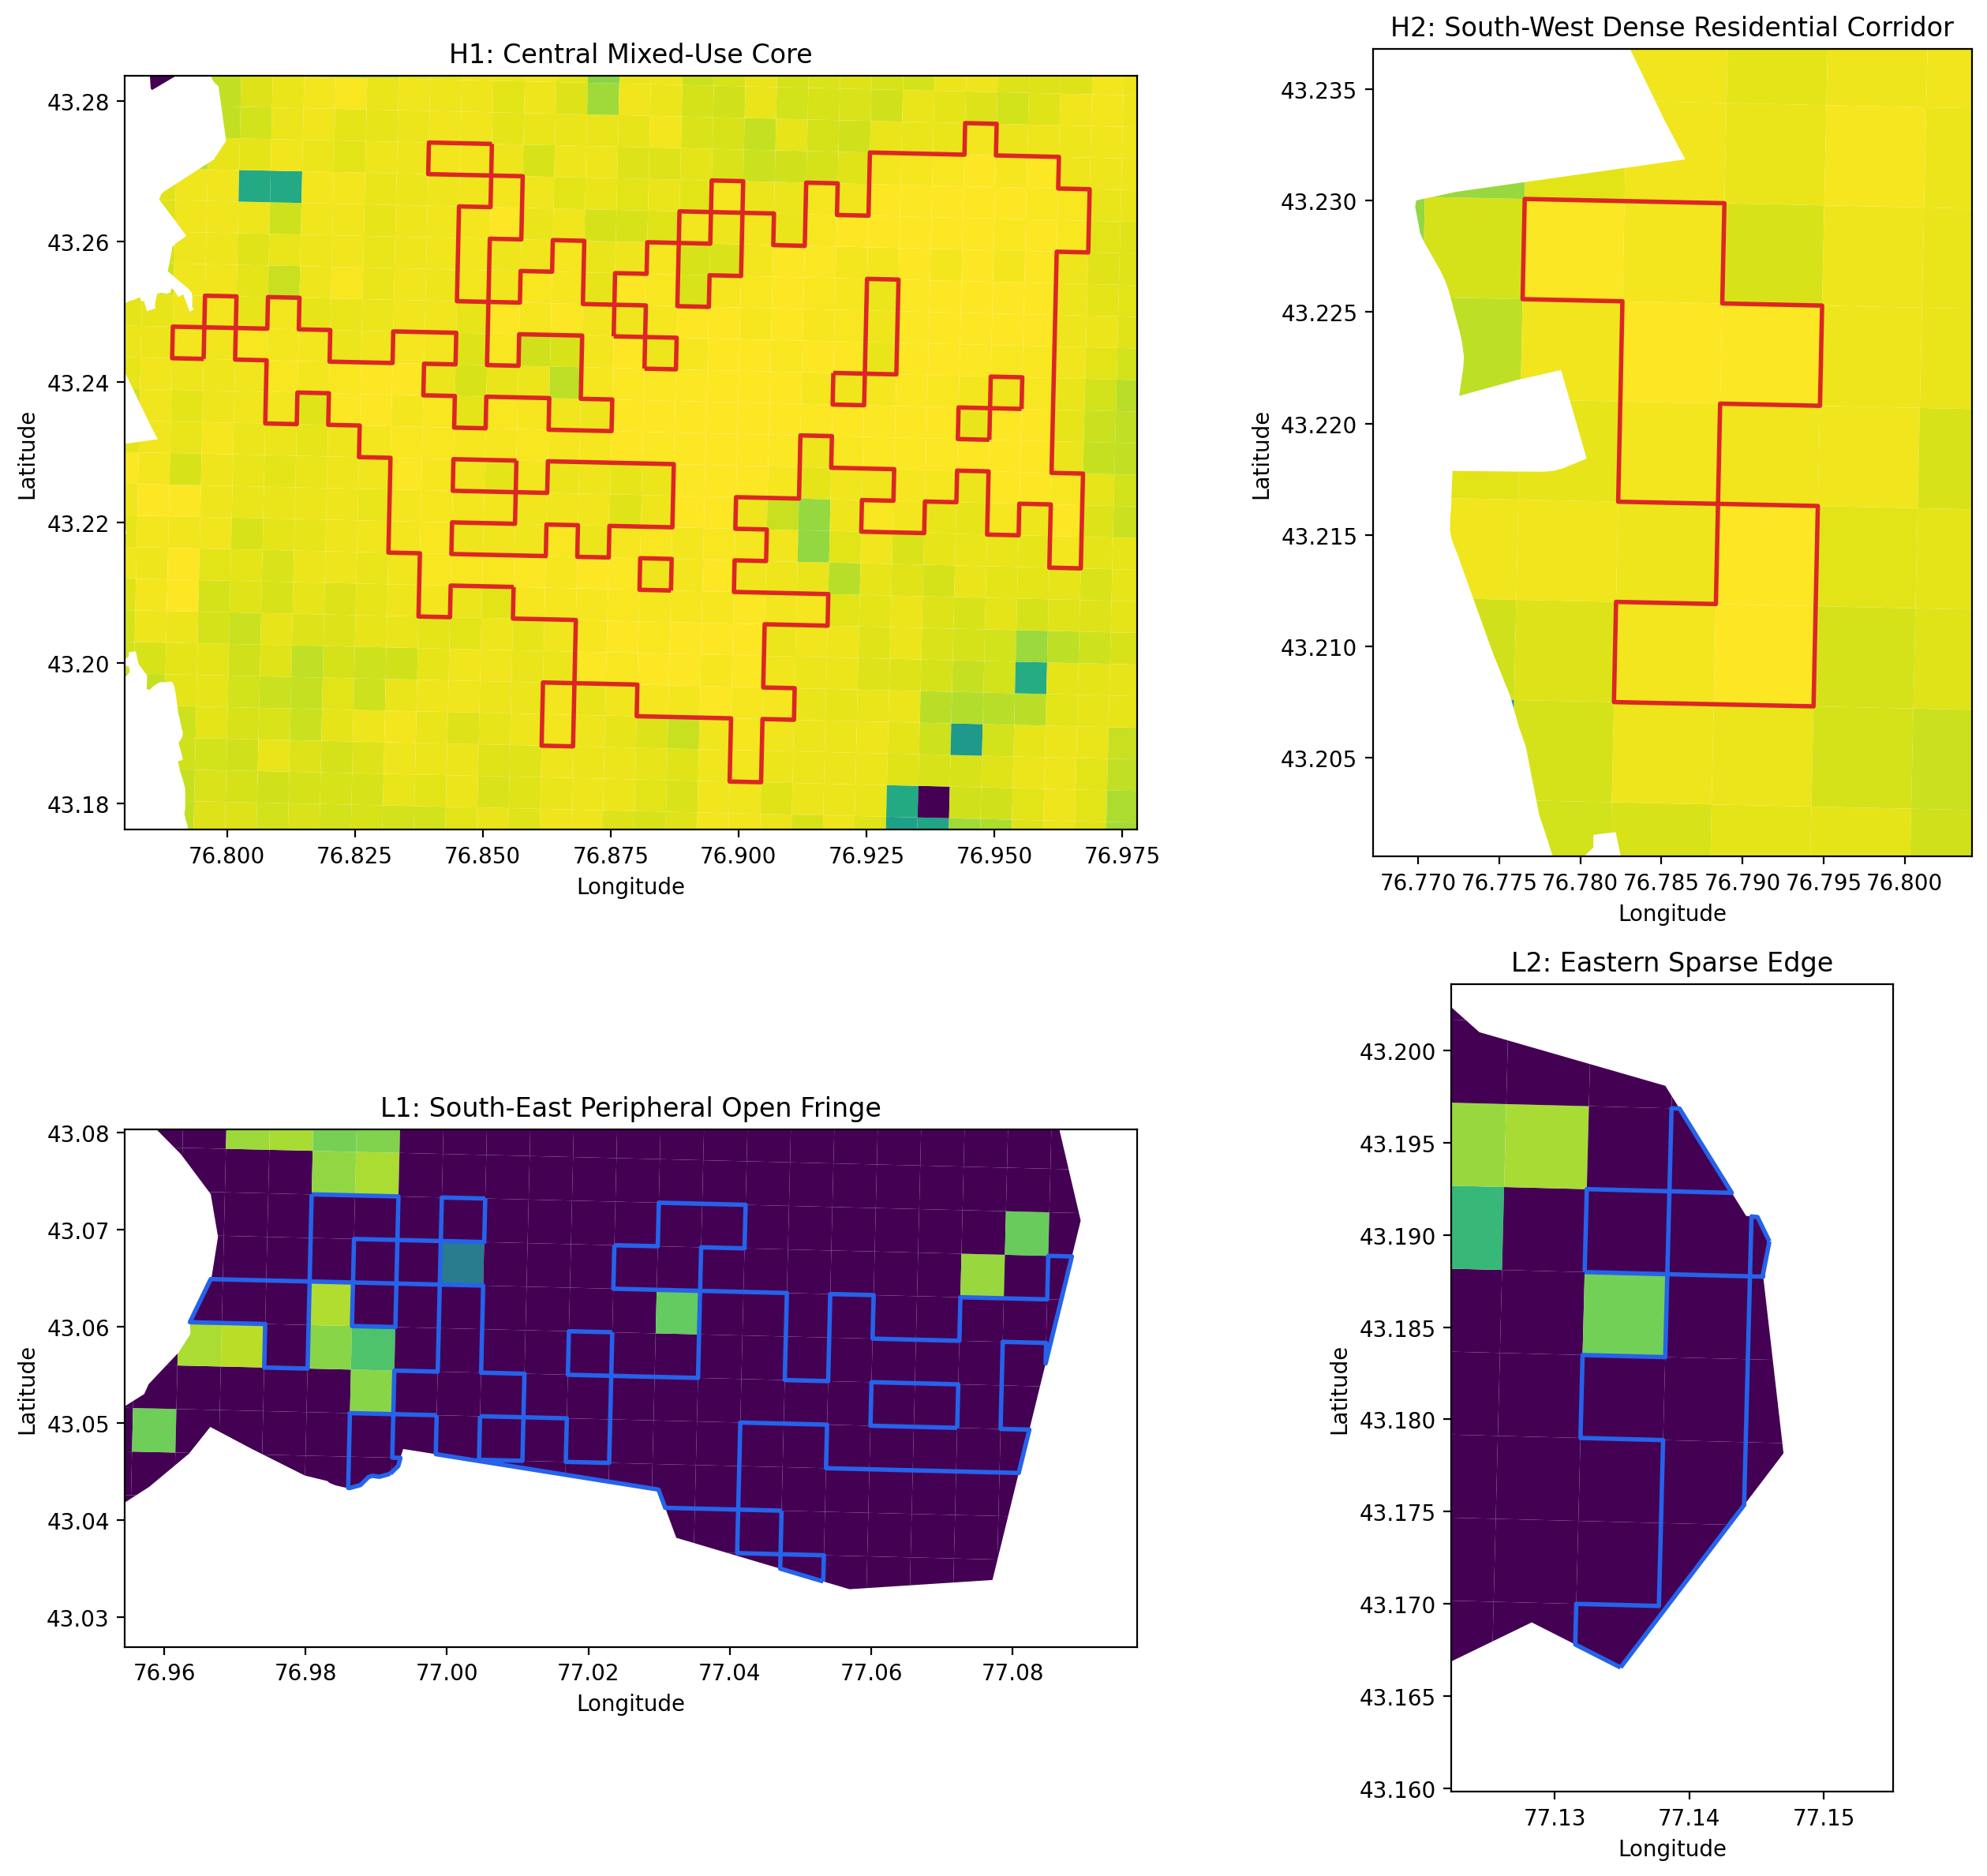
\includegraphics[width=\textwidth]{figures/figure_qualitative_cases_almaty.png}
    \caption{Almaty curated cases}
\end{subfigure}
\hfill
\begin{subfigure}[t]{0.48\textwidth}
    \centering
    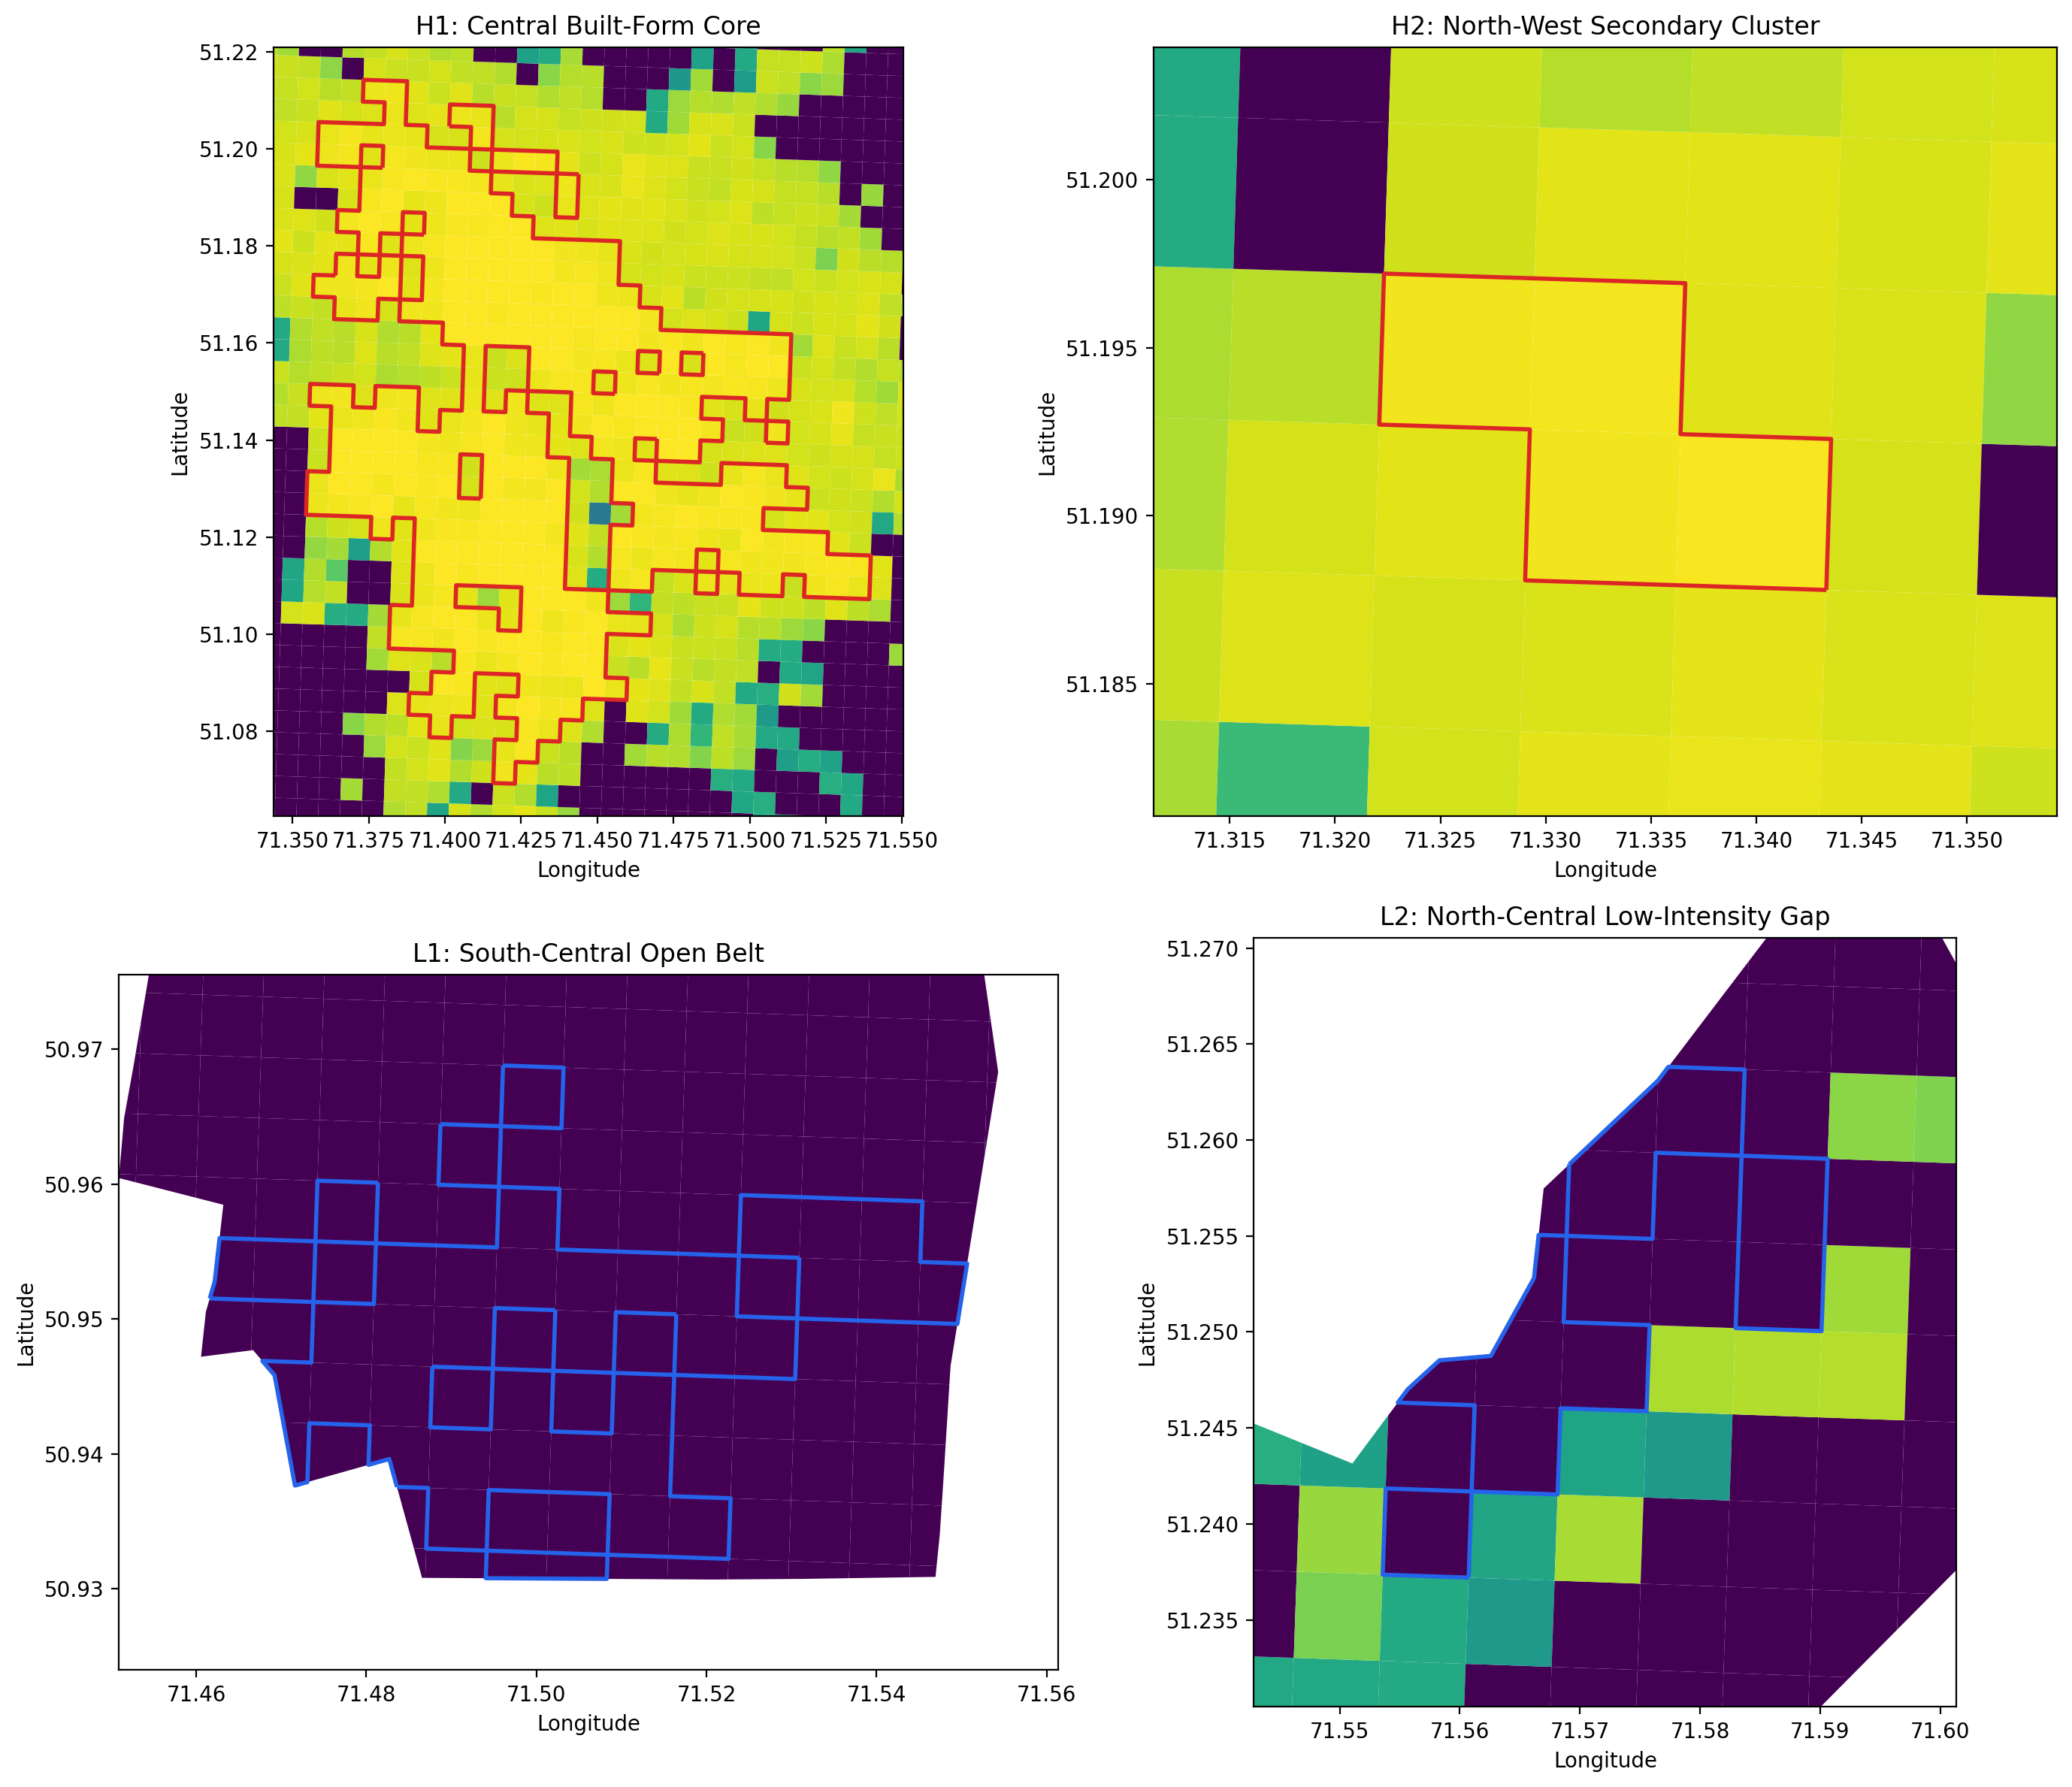
\includegraphics[width=\textwidth]{figures/figure_qualitative_cases_astana.png}
    \caption{Astana curated cases}
\end{subfigure}
\caption{Detailed qualitative hotspot and coldspot cases retained as supplement material. These panels are interpreted as plausibility evidence rather than as cell-level truth validation.}
\end{figure}

\section{S6. Example surface maps}

\begin{figure}[H]
\centering
\begin{subfigure}[t]{0.48\textwidth}
    \centering
    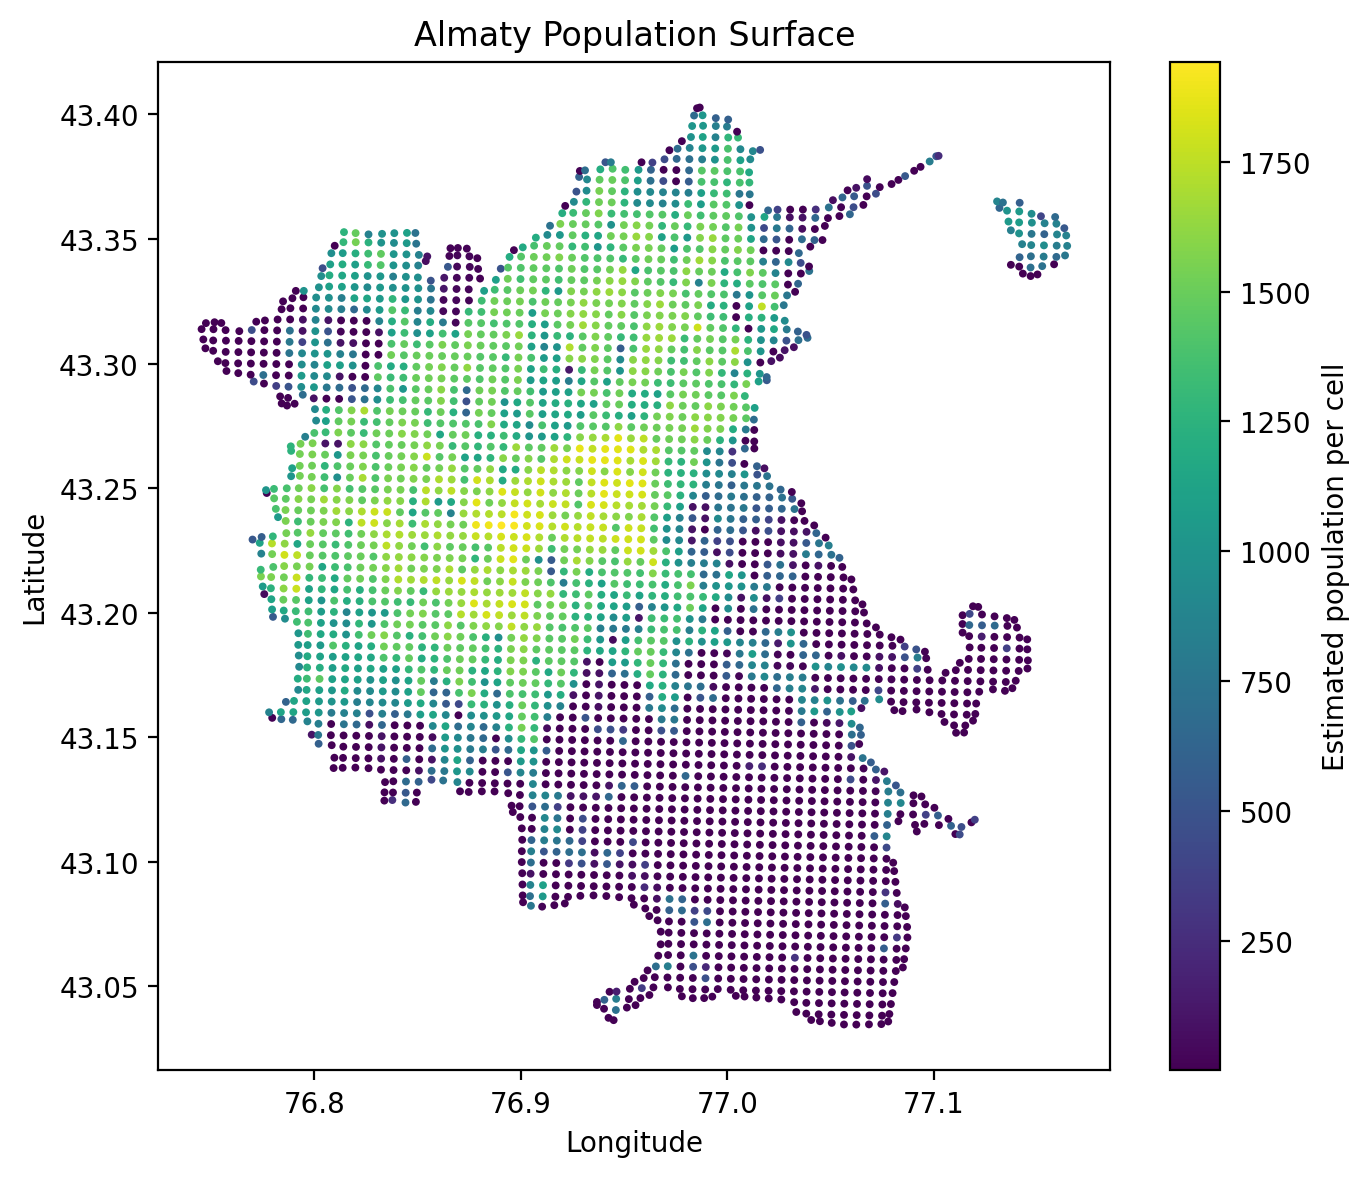
\includegraphics[width=\textwidth]{figures/figure_surface_almaty.png}
    \caption{Almaty surface example}
\end{subfigure}
\hfill
\begin{subfigure}[t]{0.48\textwidth}
    \centering
    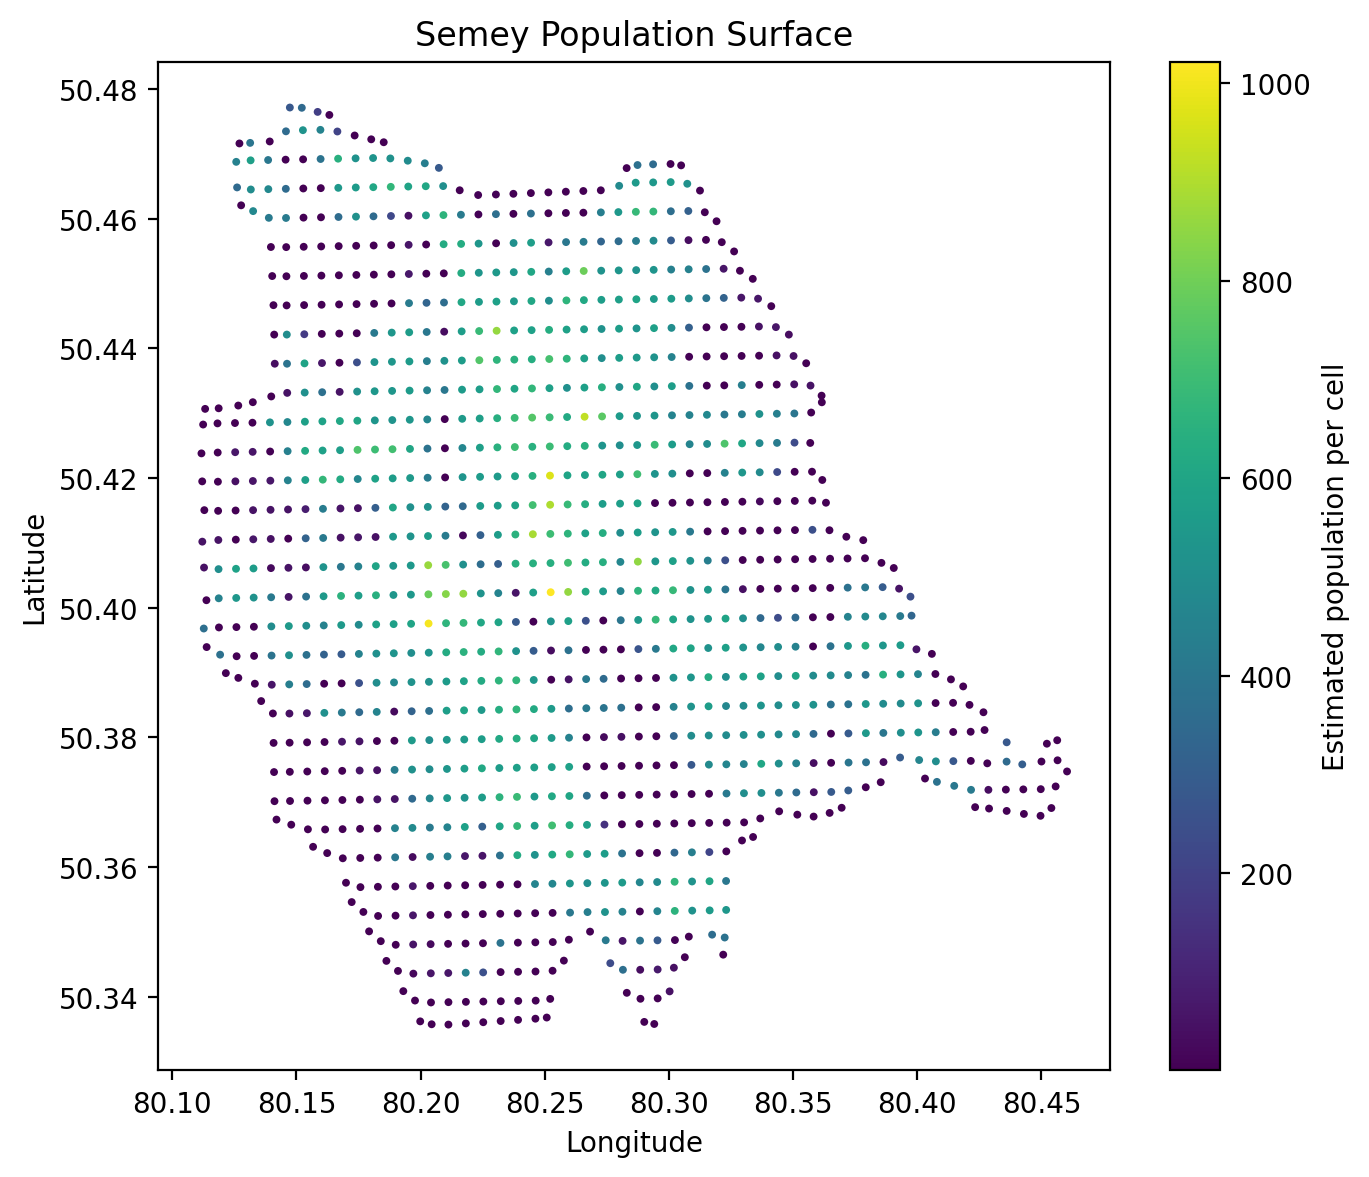
\includegraphics[width=\textwidth]{figures/figure_surface_semey.png}
    \caption{Semey surface example}
\end{subfigure}
\caption{Additional example proxy population surfaces retained as supplementary visual material.}
\end{figure}

\section{S7. Expanded supporting tables}

The following CSV-derived tables are retained as supplement material:

\begin{itemize}
\item \texttt{qa\_city\_summary\_table.csv}
\item \texttt{grid\_size\_city\_recommendations\_table.csv}
\item \texttt{external\_benchmark\_metrics\_table.csv}
\item \texttt{ablation\_selected\_extras\_table.csv}
\item \texttt{qualitative\_validation\_case\_table.csv}
\end{itemize}

\end{document}
